\documentclass{article}
\usepackage[english]{babel}

\usepackage[square,comma,sort,numbers]{natbib}
\usepackage{glossaries}
\usepackage{hyperref}
\usepackage{graphicx}
\usepackage{subcaption}
\usepackage{xcolor}
\usepackage{amsmath}
\usepackage[document]{ragged2e}
\usepackage{amssymb}
\usepackage{listings}
\usepackage{adjustbox}
\usepackage{multicol}
\usepackage{dirtree}
\usepackage[T1]{fontenc}
\usepackage[font=scriptsize]{caption}

\definecolor{codegreen}{rgb}{0,0.6,0}
\definecolor{codegray}{rgb}{0.5,0.5,0.5}
\definecolor{codepurple}{rgb}{0.58,0,0.82}
\definecolor{backcolour}{rgb}{0.95,0.95,0.92}

\lstdefinestyle{mystyle}{
    backgroundcolor=\color{backcolour},   
    commentstyle=\color{codegreen},
    keywordstyle=\color{magenta},
    numberstyle=\tiny\color{codegray},
    stringstyle=\color{codepurple},
    basicstyle=\footnotesize,
    breakatwhitespace=false,         
    breaklines=true,                 
    captionpos=b,                    
    keepspaces=true,                 
    numbers=left,                    
    numbersep=5pt,                  
    showspaces=false,                
    showstringspaces=false,
    showtabs=false,                  
    tabsize=2
}
 
\lstset{style=mystyle}
 
\renewcommand{\familydefault}{\sfdefault}
\setlength{\columnsep}{1cm}
\graphicspath{ {images/} }


% \makeglossaries
% \newglossaryentry{ZMP}{
  name=Zero Moment Point,
  description={A definition}
}

\title{\textbf{Capstone Report}\\Arise and walk, by Deep Deterministic Policy Gradient algorithm}
\date{\today}
\author{Guitard Alan}

\begin{document}

\maketitle

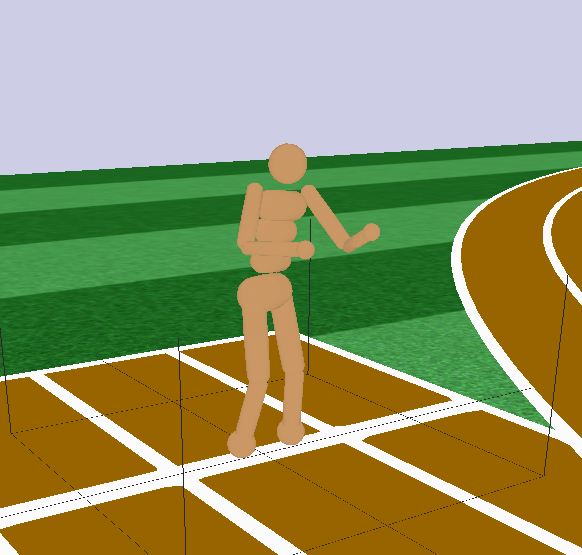
\includegraphics[width=\textwidth]{roboschoolhumanoid}
\justify

\section{Definition of the problem}

\subsection{Project Overview}
\paragraph{}
With this project, I want to tackle an important task of robotics: the ability
of a humanoid to walk. This is a really interesting problem since we, humans, learn
to walk without any feedback from another agent, just by a training process. The
parents doesn't teach anything to the kids, the kids just learns. I think this
is very interesting to build such model of artificial intelligence in order to
to understand our brain a little bit more.
\paragraph{}
The anthropologic reason is not the only reason that task is important, it is
also important to build autonomous walking robots able to progress on every
fields. There are several areas of actions: In war, such a robot will be able to
reach wounded soldier to give medical treatment or bring the soldier back to a
safe place. It will avoid a medic human to risk his life in order to do that. In
hospital, we will gain time by giving task to the walking robot so doctors and
nurses will have more time to give to the patient. In every day life, we will be
able to get near from the future described by movies like ``I-Robot''. Even if
it questions the place of the robot in human society, I think making this kind of
robot is still a goal to reach in order to send the robot in places human cannot
or with difficulty go, like to another planet.
\paragraph{}
I am talking about walking but a neural network able to make a robot walk sure
will be able to tackle another difficult task. The difficulty in those task is
their continuous observation spaces. Indeed, in order to make a robot walk, we
have two possibilities. The first one is to learn over pixels of the
environment. I didn't choose this one because I don't think a human learn to
walk from its sight but rather from its body. That why I chose to watch the
position of its joints. With pixels, we will able to train the humanoid to watch
its steps but only after it is able to walk.

\subsection{Problem Statement}
\paragraph{}
The goal of this project, precisely, is to train a 3D avatar to walk forward on
a plane fields. I will use OpenAI Gym \cite{1606.01540} as an interface to the environment
because it gives a simple and general way to use all kind of environment. For
3-dimensional avatar, it provides a binding for Mujoco library but since
this library is paid, I will use a free similar one called
Roboschool\footnote{\href{https://github.com/openai/roboschool}
  {https://github.com/openai/roboschool}} which proposes
few environments among the one I will use, RoboschoolHumanoid-v1. I am planning
to use Reinforcement Learning to tackle this task with the Deep Deterministic
Policy Gradient algorithm (\citeauthor{journals/corr/LillicrapHPHETS15}), an
actor-critic algorithm. It is ``Deep'' because the actor and the critic is
designed with deep neural networks. This algorithm is mostly used when the
environment is a continuous space and since this environment never changes in
our case (it is a plane field without changes), we can use a deterministic policy. 

\paragraph{Actor Critic algorithm}

In Reinforcement Learning, many algorithms uses an action-value function.
It is a function which returns the value of an action $a$ from a state $s$
following a policy $\mu$. It is defined like this: 
  
\begin{equation}
  Q^\mu(s_t,a_t) = \mathbb{E}_{r_t,s_{t+1}\sim{E}}[r(s_t,a_t) + \gamma
  Q^\mu(s_{t+1}, \mu(s_{t+1}))]
\end{equation}

Besides that, the policy is the map of probabilities for an agent to go
to state $s_{t+1}$ from state $s$ by the action $a$:

\begin{equation}
  \mu(s,a) = P(a_t=a|s_t=s)
\end{equation}

The idea of actor-critic algorithms is to use the action-value function as a
critic which will give the $Q$ value of the action taken by the agent at each time
step. The higher the $Q$ is, the more the reward the agent will get by taking
that action in that state. The agent, here called the actor, will follow a
policy $\mu$ in order to chose the action and that policy will be updated by the
output of the critic. In Layman's terms, the actor is a child playing in the
sandbox and the critic is the parent watching him. When the child make an action
that may lead to a bad state, the parent gives him a bad reward in order to
change his behaviour (policy).

\subsection{Metrics}

\paragraph{}
I will need two set of metrics because I have two kind of session for the body:
it can walk and fail to stand or it can walk without falling. When the avatar
will fall, I will restart the session, because to teach it to stand up is
another kind of problem.
\paragraph{}
At the beggining of the training, the body will fall and fall again very quickly.
So my metrics during that period will be the amount of time step it took before
failing, the distance of the gravity center from the floor, the reward per
action and the global average reward. Since the actor and critic are neural
networks, I will also plot the loss of the critic network and their weights and
biases, to check if it is changing over times. With these informations, I will
be able to tell if my models is training well or if I have to adjust my parameters.
When the body will start to have less fall, some of these metrics will not be
informative anymore. I have to find metrics to evaluate the gait of the walk.
For that, I will plot the angle of the current body position from the start
position in respect to the axe the avatar will try to follow. 

\newpage
\section{Analysis}

\subsection{Data Exploration: RoboschoolHumanoid-v1}

\subsubsection{Observation space}
\label{subsubsec:obs_space}

\paragraph{Definition} An observation space, or state space, is the shape and
the possible values an environment state could have. If the state is not
continuous, we can calculate the state space by counting all possible values.
For example, in a tic-tac-toe game, every square have 3 states so the state
space is $3^9 = 19,683$. Here, our state is continuous, meaning that our possible
values stands in a range. We can then just describe values and specify the range.

\paragraph{}
Our environment has an observation space of 44 float values in the range [-5,
5] which is a concatenation a three vectors described as follows:
\begin{itemize}
\item{\textbf{more}: It is a vector of 8 values defined as follows:
    \begin{itemize}
    \item{The distance between the last position of the body and the current one.}
    \item{The sinus of the angle to the target.}
    \item{The cosinus of the angle to the target.}
    \item{The three next values is the X, Y and Z values of the matrix multiplication between
        \begin{itemize}
        \item{\[\left(
                \begin{matrix}
                  \cos(-yaw) & -\sin(-yaw) & 0 \\
                  \sin(-yaw) & \cos(yaw) & 0 \\
                  0 & 0 & 1
                \end{matrix}\right)
            \]}
        \item{The speed vector of the body.}
        \end{itemize}}
    \item{The roll value of the body}
    \item{The pitch value of the body}
    \end{itemize}}
\item{\textbf{j}: This is the current relative position of the joint described earlier and their current speed. The position is in the even position, and the speed in the odds (34 values).}
\item{\textbf{feet\_contact}: Boolean values, 0 or 1, for left and right feet, indicating if the respective feet is touching the ground or not.}
\end{itemize}

\subsubsection{Action space}

\paragraph{Definition} An action space is like observation space but for action
an actor can take. In the tic-tac-toe example, the actor has 9 possible actions,
which is playing in one of the square. 
\paragraph{}
The action space is a vector of 17 float values in the range [-1, 1]. Each
value corresponds to the joints of the avatar by this order in the 
\href{https://github.com/openai/roboschool/blob/master/roboschool/mujoco_assets/humanoid_symmetric.xml}{XML}
file:
\begin{multicols}{2}
  \begin{itemize}
  \item{abdomen\_y}
  \item{abdomen\_z}
  \item{abdomen\_x}
  \item{right\_hip\_x}
  \item{right\_hip\_z}
  \item{right\_hip\_y}
  \item{right\_knee}
  \item{left\_hip\_x}
  \item{left\_hip\_z}
  \item{left\_hip\_y}
  \item{left\_knee}
  \item{right\_shoulder1}
  \item{right\_shoulder2}
  \item{right\_elbow}
  \item{left\_shoulder1}
  \item{left\_shoulder2}
  \item{left\_elbow}
  \end{itemize}
\end{multicols}
  At each step, these values are applied to all the joints of the body by the code
\begin{lstlisting}[language=Python]
for n,j in enumerate(self.ordered_joints):
    j.set_motor_torque( self.power*j.power_coef \
                         *float(np.clip(a[n], -1, +1)) )
\end{lstlisting}

in the \verb?apply\_action? function in the class which extends the
\verb?gym.Env? class (\verb?RoboschoolMujocoXmlEnv?) to set the torque value
into the respective motor.

\subsubsection{Reward}

\paragraph{Definition} A reward is a value given the information if the action
was good or not given the state. The definition of the reward function is a
critical aspect of reinforcement learning since it is the one who gives the most
valuable information during the training.
\paragraph{}
The reward is a sum of 5 computed values: \begin{itemize}
  \item{\textbf{alive}: -1 or +1 wether is on the ground or not}
  \item{\textbf{progress}: potential minus the old potential. The potential is defined by
    the speed multiplied by the distance to target point, to the negative.}
  \item{\textbf{electricity\_cost}: The amount of energy needed for the last action}
  \item{\textbf{joints\_at\_limit\_cost}: The amount of collision between joints of body
      during the last action}
  \item{\textbf{feet\_collsion\_cost}: The amount of feet collision taken during the last action}
  \end{itemize}

\subsection{Exploratory Visualization}

% NOT WHAT ASKED FOR
% To visualize the exploration, we can simply use the render function of the gym
% environment which uses \verb?Roboschool? library to create the 3D plane and
% humanoid such as show in the figure \ref{fig:roboschoolhumanoid}.  

% \begin{figure}[ht]
%   \centering
%   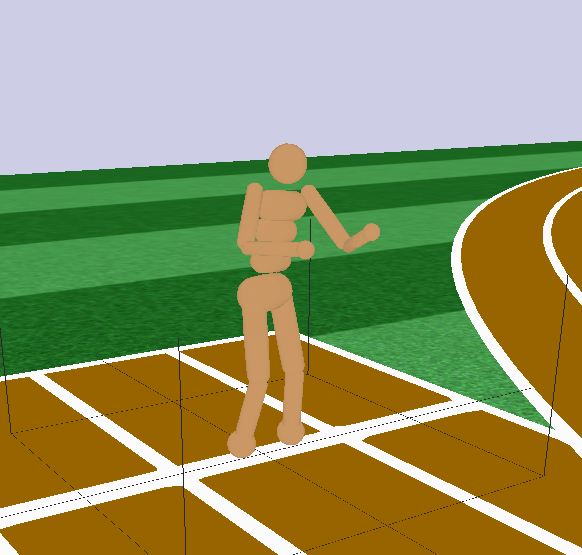
\includegraphics[width=.5\textwidth]{roboschoolhumanoid}
%   \caption{Roboschool environment}
%   \label{fig:roboschoolhumanoid}
% \end{figure}

\subsection{Algorithm and Techniques}

\paragraph{Deep Deterministic Policy Gradient}

In DDPG, instead of compute manually the $Q$ value and the $\mu$, we
use neural networks, one for the actor and one for the critic. The figure
\ref{fig:actor-critic} shows how such a model can train.

\begin{figure}[ht]
  \centering
  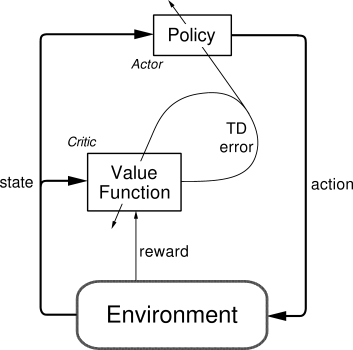
\includegraphics[width=.5\textwidth]{actor-critic}
  \caption{First, the environment gives the first state to the actor and it chose the
action following the policy. The action is given back to the environment and a
reward is computed, meaning how good the action was for that state, and sent to
the critic network. The critic computes the $Q$ value of that action by
minimizing the loss and gives the error to the actor in order to let him train
on it.}
  \label{fig:actor-critic}
\end{figure}

The Temporal Difference learning (TD Error in the figure) is a machine learning
technique to, basically, let a network able to train with a little guess of the
future. In our case of walking, the critic should not only see the next state
but also estimate the chance the actor has to fall because of the action it
took. To do that, we will use target actor and target critic network. It is, at
the beggining, a copy of the actor and the critic but we will use these networks
to compute the target action for a state and $Q_{t+1}$ and, at each time steps,
we will update their weights $\theta^{Q'}$ with the actual network weights
$\theta^Q$ by the following formula called ``soft update'':  

\begin{equation}
\theta^{Q'} \leftarrow \tau\theta^Q + (1 - \tau)\theta^Q
\end{equation}

Not using target networks will cause divergence and none of the model will learn
a good policy or a good $Q$-value function.
\paragraph{}
We need to also design a Replay buffer to store transition $(s_t, a, r,
s_{t+1})$ and train over minibatch of random transition. In that way, we break
temporal correlations between transition and minimize variance between our
possible bad predictions.
\paragraph{}
A last thing we need to introduce is exploration noise. We want to add some noise to the
action the actor take during training in order to let it explore its world with
some randomness. A good way to compute noise is the Ornstein–Uhlenbeck process,
which is also known as Brownian motion. 

\begin{figure}[ht]
  \centering
  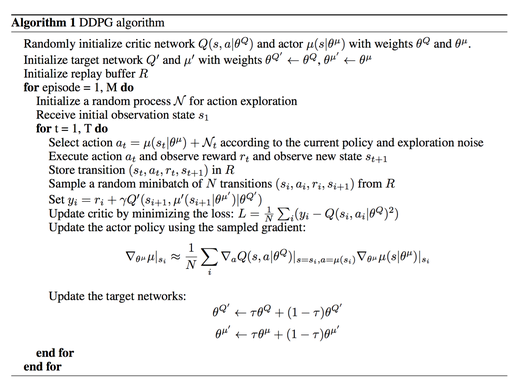
\includegraphics[width=\textwidth]{algoDDPG}
  \caption{Algorithm from \citeauthor{journals/corr/LillicrapHPHETS15} paper}
  \label{fig:algoDDPG}
\end{figure}

The figure \ref{fig:algoDDPG} describes the algorithm in a pseudo-code. The
reader can see that the actor doesn't learn the classical way, i.e. by
minimizing its loss. Instead of that, its weights is updated with the gradient
of the critic network after it trained. 

\subsection{Benchmark}

The most basic benchmark we have to test is the random benchmark. What will
happen in a worse case scenario ? 

\begin{figure}[ht]
  \centering
  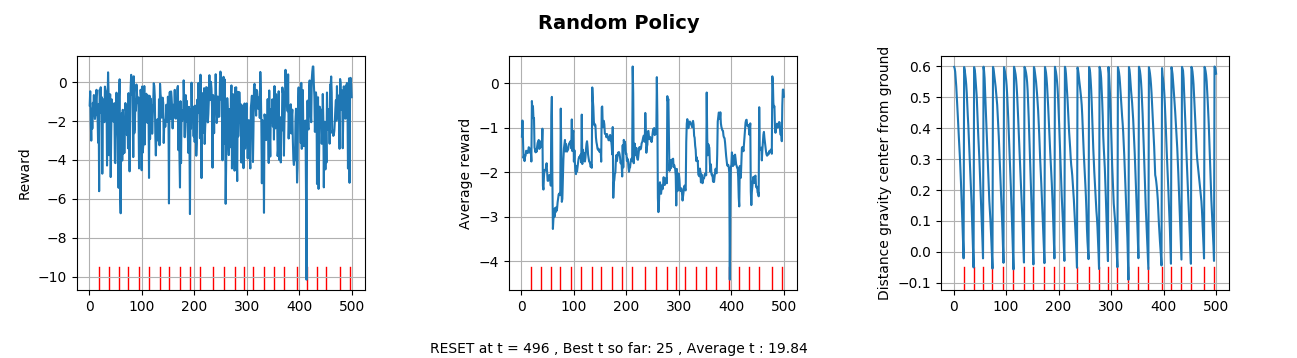
\includegraphics[width=\textwidth]{randompolicy}
  \caption{Random Policy}
  \label{fig:randompolicy}
\end{figure}

The figure \ref{fig:randompolicy} shows that the agent fall and fall again,
without any chance to stand. The relevant information here is the average
reward. The average reward of the random policy over 500 epochs is around 20 and
the agent never lives more than 30 epochs.
\paragraph{}
Now we have a low benchmark, we have to dig into previous work of the community
in order to find the state-of-the-art paper for that task. The work of
\citeauthor{journals/corr/LillicrapHPHETS15} in their paper called
\textit{Continuous control with deep reinforcement Learning} does not show
results with a humanoid environment but they did reach a good policy for 2d
walker. Another more recent studies\cite{GuLilGhaTurLev17} shows results of
different algorithm including DDPG. 

\begin{figure}[ht]
  \centering
  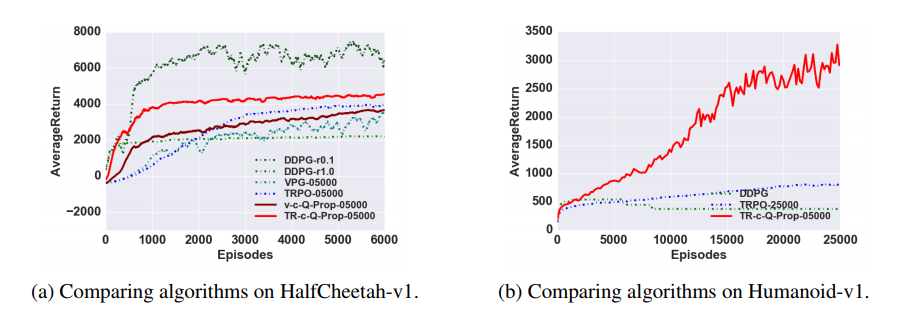
\includegraphics[width=\textwidth]{benchmark}
  \caption{Average return over episodes in HalfCheetah-v1 and Humanoid-v1 during
    learning, comparing Q-Prop against other model-free algorithms. Q-Prop with
    vanilla policy gradient outperforms TRPO on HalfCheetah. Q-Prop
    significantly outperforms TRPO in convergence time on Humanoid.}
  \label{fig:benchmark}
\end{figure}

The figure \ref{fig:benchmark} emphases that maybe DDPG is not a good choice to
such a complex environment like Humanoid because DDPG is really sensitive about
hyper-parameters changes. I still want to try to teach a robot to walk with that
algorithm by increasing the depth of the networks for example and see what
happened.  

\section{Methodology}

\subsection{Data Preprocessing}

The Roboschool environment is made for educational and research purpose. In that
matter, a lot of useful data preprocessing is already made. For the observation
vector, after building it as explained in section \ref{subsubsec:obs_space}, the
value is clipped between -5 and 5, meaning that if the environment provides a
value outside of these bounds, the value is set to the nearest bounds. This is
the same for action space but the value is clipped between -1 and 1. 

\subsection{Implementation}

\subsubsection{Project Structure}

I present you below the structure of my project:

\dirtree{%
.1 /.
.2 params.json.
.2 main\_walk.py.
.2 walk.
.3 agents.
.4 abstract\_env.py.
.4 ac\_policy.py.
.4 random\_policy.py.
.3 models.
.4 actor\_critic.py.
.3 utils.
.4 board.py.
.4 matplotboard.py.
.4 memory.py.
.4 noise.py.
.4 params.py.
.4 tensorboard.py.
}

In the \verb?agents? folder, the \verb?abstract_env.py? file is meant to be the
super class of every policy I could implement, managing operation that every
environment has to manage like instancing the plotting library or resetting the
environment and its variables. In the \verb?models? folder, we have our actor
and critic networks definitions. In the \verb?utils? folder, we have all classes
used by our algorithm to make it work properly like visualization class, data
structure and noise definition. The last thing I need to precise is that a lot
of parameters in my program is written in \verb?params.json? and read at
runtime. By this way, I can search for the good set of parameters without
entering into the code. I will explain in section \ref{subsubsec:hp_params} this
file precisely after my implementation description.

\subsubsection{Replay buffer}

To implement that task, I started by writing the replay buffer. I created a
class \verb?Memory? which holds a queue as a member in order to store tuple of
$(s_t, a, r, s_{t+1})$. I defined the first method as follow:

\begin{lstlisting}[language=Python]
def remember(self, state, action, reward, next_state, done, state_range=None, action_range=None)
\end{lstlisting}

The \verb?done? value is a boolean telling if the state is terminal or not. The
state and the action range is a value to normalize the respective vector between
0 and 1. I think by this way neural networks will have better performance
because input is less sparsed. If not \verb?None?, these values must be equal to
the range between low and high value (2 for action and 10 for state in our
case).\\
The second needed method to define is the one to get samples from the queue randomly:

\begin{lstlisting}[language=Python]
def samples(self, batch_size)
\end{lstlisting}

We need to get random sample, not last one or older one, but random, in order to
break their correlations which would lead to decrease the performance of the model.

\subsubsection{Neural networks: Actor and Critic}

\paragraph{Keras vs Tensorflow}

In the beginning, to design my networks, I used Keras but this library is
high-level API over Theano, Tensorflow and CNTK. It means that when we use it,
we lose some control over the low-level API in order to be more readable and
easy to implement. Since I will need to compute gradients and applying it to
another networks, I understand that it will be more easy to do that in
Tensorflow and it will be a good occasion to start to learn it.

\paragraph{The Actor}

The actor model is composed by fully-connected layers followed by Rectified
Linear Unit activation function and then by batch normalization, because it
gives better training speed and efficiency. The input is a shape of 44 float
values for the state and the output is a shape of 17 float values activated by
hyperbolic tangent because the range of the action values is equal to defintion
range of the hyperbolic tangent, [-1, 1].

\paragraph{The Critic}

The critic model is composed by two inputs, one for the state and one for the
action. The state input is followed by several dense layers activated by ReLU
and batch normalization. The action input is followed by one layer with the same
number of node than the last layer of the state network in order to be able to
merge them. That layer is also followed by activation ReLU activation and
batch normalization. These two layers is then added and followed by the output
layer, a single-node one representing the Q-value of the state-action pair.

\paragraph{Target networks}

In our training process, when we have to do inferences from next actions or next
states, we have to use actor target network and critic target network. These
identical network has been recently shown to increase stability during the
training and decrease variance of outputs.

\subsubsection{Training}

\paragraph{The Actor}

To train the actor network, we must define operations capable of applying action
gradients computed by critic network. I have three steps:
\begin{enumerate}
\item Compute the gradients:
\begin{lstlisting}[language=Python]
self.unnormalized_actor_gradients = tf.gradients(
    self.output, self.network_params, -self.action_gradients)
\end{lstlisting}
  I called these gradients unnormalized because since we compute gradients over
  mini-batches, we need to ponderate gradients with the size of these batches.
\item Ponderate gradients:
\begin{lstlisting}[language=Python]
self.actor_gradients = list(
    map(
        lambda x: tf.div(x, self.batch_size),
        self.unnormalized_actor_gradients))
\end{lstlisting}
  Now that we have actor gradients, we can apply it to the actor variables:
\item Applying gradients:
\begin{lstlisting}[language=Python]
self.network_params = tf.get_collection(tf.GraphKeys.TRAINABLE_VARIABLES, scope=self.scope+"/model")
# ...
self.opt = tf.train.AdamOptimizer(
    self.lr).apply_gradients(
        zip(self.actor_gradients, self.network_params))
\end{lstlisting}
\end{enumerate}

\paragraph{The Critic}

I defined training operations for the critic with a mean squared error loss
function and the ADAM optimizer, with learning rate defined in parameters and
minimizing the loss.

\paragraph{Process}
Here comes the salt and pepper of Deep Deterministic Policy Gradients. I need
here to train the critic network first, computing the gradients and apply it to
the actor network. Here the complete code which is basically the implementation
of the figure \ref{fig:algoDDPG}:

\begin{lstlisting}[language=Python]
# Get samples of memory
states, actions, rewards, next_states, dones = \
    self.memory.samples(self.params.batch_size)

with tf.variable_scope("train_critic"):
    # Predicted actions
    next_actions = self.tf_session.run(
        self.target_actor_model.output,
        feed_dict={
            self.target_actor_model.input_ph: next_states
        })

    if self.params.action_range:
        next_actions = (next_actions +
                        self.params.action_range/2
        ) / self.params.action_range

    # Compute the Q+1 value with next s+1 and a+1
    Q_next = self.tf_session.run(
          self.target_critic_model.Q, 
          feed_dict={
              self.target_critic_model.input_state_ph: next_states,
              self.target_critic_model.input_action_ph: next_actions
          })

    # gamma is the discounted factor
    Q_next = self.params.gamma * Q_next * (1 - dones)
    Q_next = np.add(Q_next, rewards)

    # Train the critic network and get gradients
    feed_critic = {
        self.critic_model.input_state_ph: states,
        self.critic_model.input_action_ph: actions,
        self.critic_model.true_target_ph: Q_next
    }
    self.critic_loss, _, critic_action_gradient = \
        self.tf_session.run(
            [self.critic_model.loss, self.critic_model.opt,
             self.critic_model.action_gradients],
        feed_dict=feed_critic)

    with tf.variable_scope("train_actor"):
        # Train the actor network with the critic gradients
        feed_actor = {
            self.actor_model.input_ph: states,
            self.actor_model.action_gradients: \
                 critic_action_gradient[0]
        }
        self.actor_loss, _ = self.tf_session.run(
            [self.actor_model.loss,
             self.actor_model.opt],
             feed_dict=feed_actor)

    with tf.variable_scope("soft_update"):
        # Update target network
        self._update_target_network()
\end{lstlisting}

Here is the step by step explanation:
\begin{itemize}
\item We get temporally not-correlated batch from memory.
\item We compute next actions with next states.
\item We compute the expected reward $Q_{next}$ with next states and next actions.
\item We ponderate (or ignoring if the state is final) by the gamma parameters,
  i.e the discounted factor.
\item We use it as a label to train the critic network and get gradients.
\item We can then apply these gradients the actor to train it.
\item Finally, we update target networks with soft update function.
  \begin{lstlisting}[language=Python]
self.update_critic_target =
   [self.ct_params[i].assign(
                tf.multiply(self.c_params[i], 
                            self.params.tau) + 
                tf.multiply(self.ct_params[i],
                            1. - self.params.tau))
       for i in range(len(self.ct_params))]
  
self.update_actor_target =
   [self.at_params[i].assign(
                tf.multiply(self.a_params[i], 
                            self.params.tau) +
                tf.multiply(self.at_params[i], 
                            1. - self.params.tau))
       for i in range(len(self.at_params))]
  \end{lstlisting}
\end{itemize}

\subsubsection{Noise}

In my first implementation, I used a $\epsilon$-greedy algorithm to explore the
environment. It was a decaying asymptotic-to-zero function used to generate less
and less random actions over time. But then I discovered noise function to
reduce variance and increase stability over taken actions, like
Ornstein-Uhlenbeck noise. It computes a vector of float equal to the shape
passed in parameters and we can add it to the action given by the actor.

\subsubsection{The Agent}

Here is the main loop of the program:

\begin{lstlisting}[language=Python]
for j in range(self.params.epochs):
    action = self.act(state)
    if self.params.noisy and j < self.params.noise_threshold:
        action += self.noise()

    new_state, reward, done, info = self.env.step(action)

    # Put the current environment in the memory
    # State interval is [-5;5] and action range is [-1;1]
    self.memory.remember(state, action, \ 
                         reward * self.params.reward_multiply, \
                         new_state, done, \
                         state_range=self.params.state_range, \
                         action_range=self.params.action_range)

    # Train the network
    self.train()

    # Reset the environment if done
    self.reset(done)

    # Render the environment
    self.render()

    # Plot needed values
    self.plotting(state=state, reward=reward, \ 
                  c_loss=self.critic_loss, \
                  a_loss=self.actor_loss)

    # Change current state
    state = new_state
\end{lstlisting}

\subsubsection{Hyper Parameters}
\label{subsubsec:hp_params}

I present in this section every arguments of my programs. It was really usefull
to quickly test many hyper parameters in order to see how does it affects the
training.

\begin{table}[ht]
  \centering
  \begin{adjustbox}{width=1\textwidth}
    \begin{tabular}{ |c|c|c| }
      \hline
      \textbf{Name} & \textbf{Description} & \textbf{Value for training} \\
      \hline
      device & Choose CPU or GPU to perform TF operation & \verb?gpu? \\
      reset & Reset the environment at final states & \verb?true? \\ 
      render & Render the environment\footnotemark & false \\
      plot & Choose the plotting library & \verb?tensorflow? \\
      train & Train network & \verb?true? \\
      noisy & Add noise to action outputs & \verb?true? \\
      load\_weights & Load previously saved weights & \verb?false? \\
      batch\_size & Number of samples to train from the momery & 128 \\
      epochs & Number of epochs & 1000 \\
      pass\_per\_epoch & Number of action during one epoch & 100 \\ 
      noise\_threshold & At which epochs the program stops adding noise to actions & 500 \\
      actor\_learning\_rate & Learning rate for the actor & 0.0001 \\
      critic\_learning\_rate & Learning rate for the critic & 0.001 \\
      actor\_batch\_norm & Add batch normalization after dense layers of the actor network & \verb?true? \\
      critic\_batch\_norm & Add batch normalization after dense layers of the critic network & \verb?true? \\
      tau & Used in soft target update function & 0.001 \\
      gamma & Discounted factor & 0.99 \\
      actor\_layers & Structure of actor network, depth and number of units in each layer & \verb?[400, 300]? \\
      critic\_layers & Structure of critic network, depth and number of units in each layer & \verb?[400, 300]? \\
      action\_range & Size of the action range to normalize it between 0 and 1 & 2 \\
      state\_range & Size of the state range to normalize it between 0 and 1 & 10 \\
      reward\_multiply & Multiply every reward with to reward more when good action is taken and less when a bad one is taken. & 1 \\
      dropout & percent of dropout to use after dense layers & 0 \\
      \hline
    \end{tabular}
  \end{adjustbox}
  \caption{Hyper parameters description and definition for training purpose}
  \label{tab:hyperparams}
\end{table}

\footnotetext{Roboschool has a bug which lead to give vector of \textit{inf} after the second reset when rendering, so when I train the networks, I don't render it.}

\subsection{Refinement}

\subsubsection{Noise}

To find the best tuning for my training, I changed the way I added the noise
into the action, the learning operation of my actor network and its layer
defintion. For the noise, I added it every steps. It then produces a bad
training making the loss of the critic network going up at around 350 steps
(Fig. \ref{fig:noise_600}).

\begin{figure}[ht]
  \begin{subfigure}[t]{.5\textwidth}
    \centering
    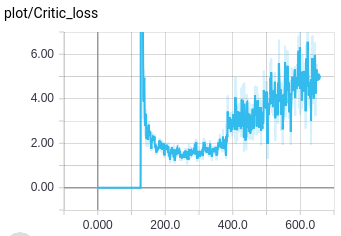
\includegraphics[width=1.\textwidth]{plot_noise_600}
    \caption{Training with noise every steps until the epoch 600}
    \label{fig:noise_600}
  \end{subfigure}%
  ~
  \begin{subfigure}[t]{.5\textwidth}
    \centering
    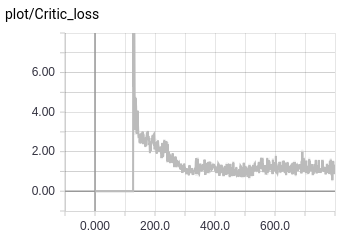
\includegraphics[width=1.\textwidth]{plot_noise_350}
    \caption{Training with noise every steps until the epoch 350}
    \label{fig:noise_350}
  \end{subfigure}
  \caption{Affect of the noise on the training process.}
\end{figure}

We can see in the figure that the noise is too much after around 350 epochs, so I changed
the parameter \verb?noise_threshold? to 350 and the result is shown in Fig. \ref{fig:noise_350}.
It shows that removing the noise at the epoch 350 remove the divergence of the loss. Henceforth,
we can interprete from the stagnation of the loss that the agent doesn't learn anymore.

\subsubsection{Network definition} 

Thanks to the architecture of my code, I am able to change the model of the networks easyly so I
tuned these parameter a lot. A lot of paper written about DDPG \cite{journals/corr/LillicrapHPHETS15}
\cite{DBLP:journals/corr/abs-1801-10425} used layers of 400 and 300 units with action added at the second
layer in the critic networkd. I then decided to follow that benchmark since it gave good results with
a lot of environment. In order to have a learning more efficient and to see how a modification would effect,
I changed the depth or the number of units. I found out that decreasing the number of units doesn't affect
the quality of the learning but decrease the speed and building the networks deeper make the critic loss
diverges very fast.

\section{Results}

\subsection{Model Evaluation and Validation}

\subsection{Justification}

\section{Conclusion}

\subsection{Free-Form Visualization}

\subsection{Reflection}

\paragraph{}
To tackle the problem, I first learned how Deep Deterministic Policy Gradients works by reading
scientific paper on that subject. I then started my implementation starting by the replay buffer
and then the DDPG algorithm itself. I added soft target update and noise addition after. Seeing
that results was not good and resolving coding mistakes (which took me a lot of time as Tensorflow
was new to me), I started to read more scientific paper and try their results with their model
architecture and their parameters. Without any more good results, it could be for two reasons:
either in some ways I have a problem in my implementation of DDPG and the update of my gradients,
either I don't have enough power on my machine to see results. The paper from
\citeauthor{journals/corr/LillicrapHPHETS15} says that DDPG has the inconvenient to be efficient
after a lot of training epochs. The first thing I wanted to test is to validate the implementation
with a more simpler environment so I tested it on the CartPole environment.

\paragraph{}
The most interesting part of the project was to see how the changes in my implementation in terms
of algorithm and parameters could change the behavior of the actor. It was also really interesting
to learn techniques scientist often use to increase stability, performance or quality of results
like noise addition or soft target update. Implementing the Deep Deterministic Policy Gradients
was also really enriching because I learned to use Tensorflow and working directly with weights,
biases and gradients and by that way increased my knowledge over how deep learning is working
mathematically (which is rather dificult to understand when we just read the theory without
actually using it). Contrary, the most difficult part was to actually validate my network. The
difficulty came from the fact that I defined my network as in the paper I read and I had trouble
having proper results. 

\subsection{Improvement}

In terms of coding, a good improvement would be to be able to launch the training over a cloud,
like AWS from Amazon or CloudML from Google. The training would be very faster and the validation
of the model as well. About the algorithm I am using, DDPG, \citeauthor{GuLilGhaTurLev17} shows
that Q-prop is more suitable for a 3d walking agent because it is more stable than DDPG during
training. It would be intersting to actually validate that statement.

\bibliography{report}
\bibliographystyle{plainnat}

\end{document}